\documentclass[]{article}
\usepackage{lmodern}
\usepackage{amssymb,amsmath}
\usepackage{ifxetex,ifluatex}
\usepackage{fixltx2e} % provides \textsubscript
\ifnum 0\ifxetex 1\fi\ifluatex 1\fi=0 % if pdftex
  \usepackage[T1]{fontenc}
  \usepackage[utf8]{inputenc}
\else % if luatex or xelatex
  \ifxetex
    \usepackage{mathspec}
  \else
    \usepackage{fontspec}
  \fi
  \defaultfontfeatures{Ligatures=TeX,Scale=MatchLowercase}
\fi
% use upquote if available, for straight quotes in verbatim environments
\IfFileExists{upquote.sty}{\usepackage{upquote}}{}
% use microtype if available
\IfFileExists{microtype.sty}{%
\usepackage{microtype}
\UseMicrotypeSet[protrusion]{basicmath} % disable protrusion for tt fonts
}{}
\usepackage[margin=1in]{geometry}
\usepackage{hyperref}
\hypersetup{unicode=true,
            pdftitle={hw03},
            pdfauthor={Arlo},
            pdfborder={0 0 0},
            breaklinks=true}
\urlstyle{same}  % don't use monospace font for urls
\usepackage{color}
\usepackage{fancyvrb}
\newcommand{\VerbBar}{|}
\newcommand{\VERB}{\Verb[commandchars=\\\{\}]}
\DefineVerbatimEnvironment{Highlighting}{Verbatim}{commandchars=\\\{\}}
% Add ',fontsize=\small' for more characters per line
\usepackage{framed}
\definecolor{shadecolor}{RGB}{248,248,248}
\newenvironment{Shaded}{\begin{snugshade}}{\end{snugshade}}
\newcommand{\AlertTok}[1]{\textcolor[rgb]{0.94,0.16,0.16}{#1}}
\newcommand{\AnnotationTok}[1]{\textcolor[rgb]{0.56,0.35,0.01}{\textbf{\textit{#1}}}}
\newcommand{\AttributeTok}[1]{\textcolor[rgb]{0.77,0.63,0.00}{#1}}
\newcommand{\BaseNTok}[1]{\textcolor[rgb]{0.00,0.00,0.81}{#1}}
\newcommand{\BuiltInTok}[1]{#1}
\newcommand{\CharTok}[1]{\textcolor[rgb]{0.31,0.60,0.02}{#1}}
\newcommand{\CommentTok}[1]{\textcolor[rgb]{0.56,0.35,0.01}{\textit{#1}}}
\newcommand{\CommentVarTok}[1]{\textcolor[rgb]{0.56,0.35,0.01}{\textbf{\textit{#1}}}}
\newcommand{\ConstantTok}[1]{\textcolor[rgb]{0.00,0.00,0.00}{#1}}
\newcommand{\ControlFlowTok}[1]{\textcolor[rgb]{0.13,0.29,0.53}{\textbf{#1}}}
\newcommand{\DataTypeTok}[1]{\textcolor[rgb]{0.13,0.29,0.53}{#1}}
\newcommand{\DecValTok}[1]{\textcolor[rgb]{0.00,0.00,0.81}{#1}}
\newcommand{\DocumentationTok}[1]{\textcolor[rgb]{0.56,0.35,0.01}{\textbf{\textit{#1}}}}
\newcommand{\ErrorTok}[1]{\textcolor[rgb]{0.64,0.00,0.00}{\textbf{#1}}}
\newcommand{\ExtensionTok}[1]{#1}
\newcommand{\FloatTok}[1]{\textcolor[rgb]{0.00,0.00,0.81}{#1}}
\newcommand{\FunctionTok}[1]{\textcolor[rgb]{0.00,0.00,0.00}{#1}}
\newcommand{\ImportTok}[1]{#1}
\newcommand{\InformationTok}[1]{\textcolor[rgb]{0.56,0.35,0.01}{\textbf{\textit{#1}}}}
\newcommand{\KeywordTok}[1]{\textcolor[rgb]{0.13,0.29,0.53}{\textbf{#1}}}
\newcommand{\NormalTok}[1]{#1}
\newcommand{\OperatorTok}[1]{\textcolor[rgb]{0.81,0.36,0.00}{\textbf{#1}}}
\newcommand{\OtherTok}[1]{\textcolor[rgb]{0.56,0.35,0.01}{#1}}
\newcommand{\PreprocessorTok}[1]{\textcolor[rgb]{0.56,0.35,0.01}{\textit{#1}}}
\newcommand{\RegionMarkerTok}[1]{#1}
\newcommand{\SpecialCharTok}[1]{\textcolor[rgb]{0.00,0.00,0.00}{#1}}
\newcommand{\SpecialStringTok}[1]{\textcolor[rgb]{0.31,0.60,0.02}{#1}}
\newcommand{\StringTok}[1]{\textcolor[rgb]{0.31,0.60,0.02}{#1}}
\newcommand{\VariableTok}[1]{\textcolor[rgb]{0.00,0.00,0.00}{#1}}
\newcommand{\VerbatimStringTok}[1]{\textcolor[rgb]{0.31,0.60,0.02}{#1}}
\newcommand{\WarningTok}[1]{\textcolor[rgb]{0.56,0.35,0.01}{\textbf{\textit{#1}}}}
\usepackage{graphicx,grffile}
\makeatletter
\def\maxwidth{\ifdim\Gin@nat@width>\linewidth\linewidth\else\Gin@nat@width\fi}
\def\maxheight{\ifdim\Gin@nat@height>\textheight\textheight\else\Gin@nat@height\fi}
\makeatother
% Scale images if necessary, so that they will not overflow the page
% margins by default, and it is still possible to overwrite the defaults
% using explicit options in \includegraphics[width, height, ...]{}
\setkeys{Gin}{width=\maxwidth,height=\maxheight,keepaspectratio}
\IfFileExists{parskip.sty}{%
\usepackage{parskip}
}{% else
\setlength{\parindent}{0pt}
\setlength{\parskip}{6pt plus 2pt minus 1pt}
}
\setlength{\emergencystretch}{3em}  % prevent overfull lines
\providecommand{\tightlist}{%
  \setlength{\itemsep}{0pt}\setlength{\parskip}{0pt}}
\setcounter{secnumdepth}{0}
% Redefines (sub)paragraphs to behave more like sections
\ifx\paragraph\undefined\else
\let\oldparagraph\paragraph
\renewcommand{\paragraph}[1]{\oldparagraph{#1}\mbox{}}
\fi
\ifx\subparagraph\undefined\else
\let\oldsubparagraph\subparagraph
\renewcommand{\subparagraph}[1]{\oldsubparagraph{#1}\mbox{}}
\fi

%%% Use protect on footnotes to avoid problems with footnotes in titles
\let\rmarkdownfootnote\footnote%
\def\footnote{\protect\rmarkdownfootnote}

%%% Change title format to be more compact
\usepackage{titling}

% Create subtitle command for use in maketitle
\providecommand{\subtitle}[1]{
  \posttitle{
    \begin{center}\large#1\end{center}
    }
}

\setlength{\droptitle}{-2em}

  \title{hw03}
    \pretitle{\vspace{\droptitle}\centering\huge}
  \posttitle{\par}
    \author{Arlo}
    \preauthor{\centering\large\emph}
  \postauthor{\par}
      \predate{\centering\large\emph}
  \postdate{\par}
    \date{9/26/2019}


\begin{document}
\maketitle

{
\setcounter{tocdepth}{2}
\tableofcontents
}
\hypertarget{assignment-3-dplyrggplot-part-ii}{%
\section{Assignment 3: dplyr/ggplot Part
II}\label{assignment-3-dplyrggplot-part-ii}}

Load packages used in exercise

\begin{Shaded}
\begin{Highlighting}[]
\KeywordTok{library}\NormalTok{(tidyverse)}
\KeywordTok{library}\NormalTok{(gapminder)}
\KeywordTok{library}\NormalTok{(ggridges)}
\KeywordTok{library}\NormalTok{(scales)}
\end{Highlighting}
\end{Shaded}

\hypertarget{task-option-2-minmax-gdpcapita-in-each-continent}{%
\subsection{Task Option 2: Min/max GDP/capita in each
continent}\label{task-option-2-minmax-gdpcapita-in-each-continent}}

Group data continent then summarize the max and min values based on that
grouping. =\textgreater{} This tibble shows the minimum and maximum
value of gdpPercap of each continent in gapminder.

\begin{Shaded}
\begin{Highlighting}[]
\NormalTok{gapminder }\OperatorTok
\StringTok{  }\KeywordTok{group_by}\NormalTok{(continent) }\OperatorTok
\StringTok{  }\KeywordTok{summarize}\NormalTok{(}\DataTypeTok{max_GDPpercap =} \KeywordTok{max}\NormalTok{(gdpPercap), }\DataTypeTok{min_GDPpercap =} \KeywordTok{min}\NormalTok{(gdpPercap)) }
\end{Highlighting}
\end{Shaded}

\begin{verbatim}
## # A tibble: 5 x 3
##   continent max_GDPpercap min_GDPpercap
##   <fct>             <dbl>         <dbl>
## 1 Africa           21951.          241.
## 2 Americas         42952.         1202.
## 3 Asia            113523.          331 
## 4 Europe           49357.          974.
## 5 Oceania          34435.        10040.
\end{verbatim}

Graph each continent's min and max values for GDP over time. Achieve
this through combining two geom\_point() plots together, where one
displays minimum values, and one displays maximum values. Relabel y axis
for more clear interpretation. Identify labels for each class to supress
unneeded information, and ensure effectice interpretation of data
points.

\begin{Shaded}
\begin{Highlighting}[]
\NormalTok{gapminder }\OperatorTok\StringTok{ }
\StringTok{  }\KeywordTok{group_by}\NormalTok{(continent) }\OperatorTok
\StringTok{  }\KeywordTok{summarize}\NormalTok{(}\DataTypeTok{max_GDPpercap =} \KeywordTok{max}\NormalTok{(gdpPercap), }\DataTypeTok{min_GDPpercap =} \KeywordTok{min}\NormalTok{(gdpPercap)) }\OperatorTok
\StringTok{      }\KeywordTok{ggplot}\NormalTok{()}\OperatorTok{+}
\StringTok{      }\KeywordTok{geom_point}\NormalTok{(}\KeywordTok{aes}\NormalTok{(continent, max_GDPpercap, }\DataTypeTok{colour =} \StringTok{"blue"}\NormalTok{, }\DataTypeTok{alpha =} \FloatTok{0.5}\NormalTok{, }\DataTypeTok{size =} \DecValTok{2}\NormalTok{)) }\OperatorTok{+}
\StringTok{      }\KeywordTok{geom_point}\NormalTok{(}\KeywordTok{aes}\NormalTok{(continent, min_GDPpercap, }\DataTypeTok{colour =} \StringTok{"red"}\NormalTok{, }\DataTypeTok{alpha =} \FloatTok{0.5}\NormalTok{, }\DataTypeTok{size =} \DecValTok{2}\NormalTok{))}\OperatorTok{+}
\StringTok{        }\KeywordTok{ylab}\NormalTok{(}\StringTok{"GDP per capita"}\NormalTok{) }\OperatorTok{+}
\StringTok{        }\KeywordTok{scale_alpha}\NormalTok{(}\StringTok{""}\NormalTok{, }\DataTypeTok{labels =} \StringTok{""}\NormalTok{) }\OperatorTok{+}
\StringTok{        }\KeywordTok{scale_size}\NormalTok{(}\StringTok{""}\NormalTok{, }\DataTypeTok{labels =} \StringTok{""}\NormalTok{) }\OperatorTok{+}
\StringTok{         }\KeywordTok{scale_colour_discrete}\NormalTok{(}\StringTok{"Gdp per capita"}\NormalTok{, }\DataTypeTok{labels =} \KeywordTok{c}\NormalTok{(}\StringTok{"Maximum"}\NormalTok{, }\StringTok{"Minimum"}\NormalTok{)) }
\end{Highlighting}
\end{Shaded}

\includegraphics{hw03_files/figure-latex/T2: plot-1.pdf}

Filter through tha gapminder data, and group together continents and
years, allowing functions to be run individually to each group of
continent, for each year. This allows the analysis of average life
expectancy values for each continent over time, by grouping all
countries' data together that are within the same continent, then
grouping each of those data by year as well. \#\# Task Option 5

\begin{Shaded}
\begin{Highlighting}[]
\NormalTok{gapminder }\OperatorTok
\StringTok{  }\KeywordTok{select}\NormalTok{ (continent, year, lifeExp) }\OperatorTok
\StringTok{  }\KeywordTok{group_by}\NormalTok{ (continent, year) }\OperatorTok
\StringTok{  }\KeywordTok{arrange}\NormalTok{ (continent, year) }\OperatorTok
\StringTok{  }\KeywordTok{summarize}\NormalTok{(}\DataTypeTok{ave_lifeEXp =} \KeywordTok{mean}\NormalTok{(lifeExp))}
\end{Highlighting}
\end{Shaded}

\begin{verbatim}
## # A tibble: 60 x 3
## # Groups:   continent [5]
##    continent  year ave_lifeEXp
##    <fct>     <int>       <dbl>
##  1 Africa     1952        39.1
##  2 Africa     1957        41.3
##  3 Africa     1962        43.3
##  4 Africa     1967        45.3
##  5 Africa     1972        47.5
##  6 Africa     1977        49.6
##  7 Africa     1982        51.6
##  8 Africa     1987        53.3
##  9 Africa     1992        53.6
## 10 Africa     1997        53.6
## # ... with 50 more rows
\end{verbatim}

Plot each dataframe, isolating each continent so that average life
expectancy values can be observed over time, then compared easily
between continents. Allowing all data to be shown in the graph ensures
the reader the confidence for using a line of best-fit, which clearly
demonstrates the coarse scale changes of lifeExp over time for each
continent.

\begin{Shaded}
\begin{Highlighting}[]
\NormalTok{gapminder }\OperatorTok\StringTok{ }
\StringTok{  }\KeywordTok{ggplot}\NormalTok{(}\KeywordTok{aes}\NormalTok{(year, lifeExp, }\DataTypeTok{group =}\NormalTok{ continent, }\DataTypeTok{colour =}\NormalTok{ continent)) }\OperatorTok{+}
\StringTok{  }\KeywordTok{geom_path}\NormalTok{(}\DataTypeTok{size =} \DecValTok{2}\NormalTok{, }\DataTypeTok{alpha =} \DecValTok{1}\OperatorTok{/}\DecValTok{3}\NormalTok{) }\OperatorTok{+}
\StringTok{  }\KeywordTok{facet_wrap}\NormalTok{(}\OperatorTok{~}\StringTok{ }\NormalTok{continent, }\DataTypeTok{nrow =} \DecValTok{1}\NormalTok{, }\DataTypeTok{scales =} \StringTok{"free"}\NormalTok{) }\OperatorTok{+}
\StringTok{  }\KeywordTok{scale_colour_discrete}\NormalTok{(}\StringTok{"Continents"}\NormalTok{, }\DataTypeTok{labels =} \KeywordTok{c}\NormalTok{(country_codes)) }\OperatorTok{+}
\StringTok{  }\KeywordTok{geom_smooth}\NormalTok{(}\DataTypeTok{method =} \StringTok{"lm"}\NormalTok{) }\OperatorTok{+}
\StringTok{  }\KeywordTok{theme_bw}\NormalTok{()}
\end{Highlighting}
\end{Shaded}

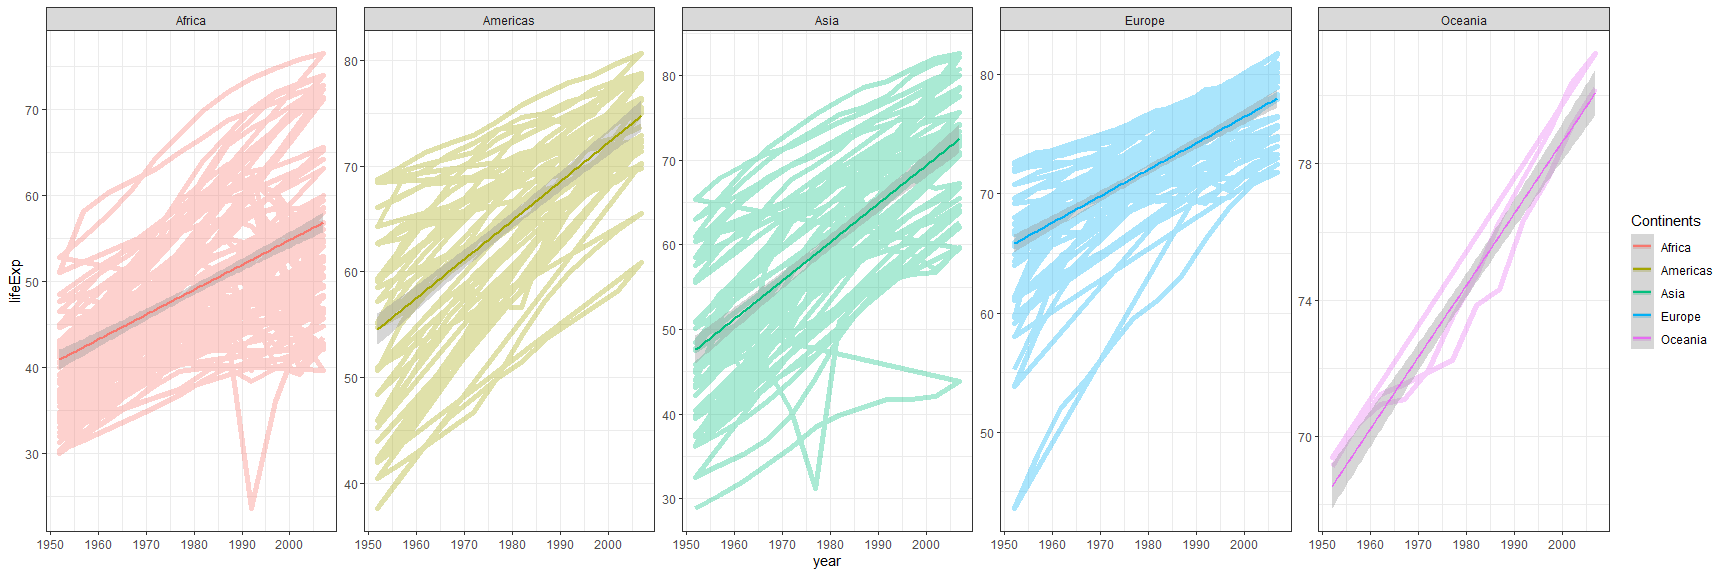
\includegraphics{hw03_files/figure-latex/t5 plot-1.pdf}

Having seen the unique gdpPercap data in class demonstration, I chose to
select only Rewanda's data for furthur investigation. I chose to
identify the increase in life expectancy for each year; and to use gross
GDP instead of gdpPercap, in order to establish a relationship between
GDP and life expectancy over time. \#\# Task Option 6

\begin{Shaded}
\begin{Highlighting}[]
\NormalTok{(Rwanda <-}\StringTok{ }\NormalTok{gapminder}\OperatorTok
\StringTok{  }\KeywordTok{filter}\NormalTok{(country }\OperatorTok{==}\StringTok{ "Rwanda"}\NormalTok{) }\OperatorTok
\StringTok{    }\KeywordTok{mutate}\NormalTok{(}\DataTypeTok{lifeExp_inc=}\NormalTok{ lifeExp }\OperatorTok{-}\StringTok{ }\KeywordTok{lag}\NormalTok{(lifeExp)) }\OperatorTok
\StringTok{    }\KeywordTok{mutate}\NormalTok{(}\DataTypeTok{GDP =}\NormalTok{ gdpPercap}\OperatorTok{*}\NormalTok{pop) }\OperatorTok
\StringTok{    }\KeywordTok{arrange}\NormalTok{(year)) }
\end{Highlighting}
\end{Shaded}

\begin{verbatim}
## # A tibble: 12 x 8
##    country continent  year lifeExp     pop gdpPercap lifeExp_inc        GDP
##    <fct>   <fct>     <int>   <dbl>   <int>     <dbl>       <dbl>      <dbl>
##  1 Rwanda  Africa     1952    40   2534927      493.      NA         1.25e9
##  2 Rwanda  Africa     1957    41.5 2822082      540.       1.5       1.52e9
##  3 Rwanda  Africa     1962    43   3051242      597.       1.5       1.82e9
##  4 Rwanda  Africa     1967    44.1 3451079      511.       1.1       1.76e9
##  5 Rwanda  Africa     1972    44.6 3992121      591.       0.5       2.36e9
##  6 Rwanda  Africa     1977    45   4657072      670.       0.400     3.12e9
##  7 Rwanda  Africa     1982    46.2 5507565      882.       1.22      4.86e9
##  8 Rwanda  Africa     1987    44.0 6349365      848.      -2.20      5.38e9
##  9 Rwanda  Africa     1992    23.6 7290203      737.     -20.4       5.37e9
## 10 Rwanda  Africa     1997    36.1 7212583      590.      12.5       4.26e9
## 11 Rwanda  Africa     2002    43.4 7852401      786.       7.33      6.17e9
## 12 Rwanda  Africa     2007    46.2 8860588      863.       2.83      7.65e9
\end{verbatim}

A graph showing the anomalies of GDP vs change in life expectancy for
Rwanda over time. Including year labels allows reader to read the data
over a time scale, despite the axes' independance to time.

\begin{Shaded}
\begin{Highlighting}[]
\NormalTok{Rwanda }\OperatorTok
\StringTok{  }\KeywordTok{ggplot}\NormalTok{(}\KeywordTok{aes}\NormalTok{(GDP, lifeExp_inc)) }\OperatorTok{+}
\StringTok{      }\KeywordTok{geom_point}\NormalTok{() }\OperatorTok{+}
\StringTok{  }\KeywordTok{scale_x_log10}\NormalTok{(}\DataTypeTok{labels =}\NormalTok{ scales}\OperatorTok{::}\KeywordTok{comma_format}\NormalTok{()) }\OperatorTok{+}
\StringTok{  }\KeywordTok{geom_text}\NormalTok{(}\KeywordTok{aes}\NormalTok{(}\DataTypeTok{label=}\NormalTok{year),}\DataTypeTok{hjust=}\DecValTok{0}\NormalTok{, }\DataTypeTok{vjust=}\DecValTok{1}
\NormalTok{            )}
\end{Highlighting}
\end{Shaded}

\begin{verbatim}
## Warning: Removed 1 rows containing missing values (geom_point).
\end{verbatim}

\begin{verbatim}
## Warning: Removed 1 rows containing missing values (geom_text).
\end{verbatim}

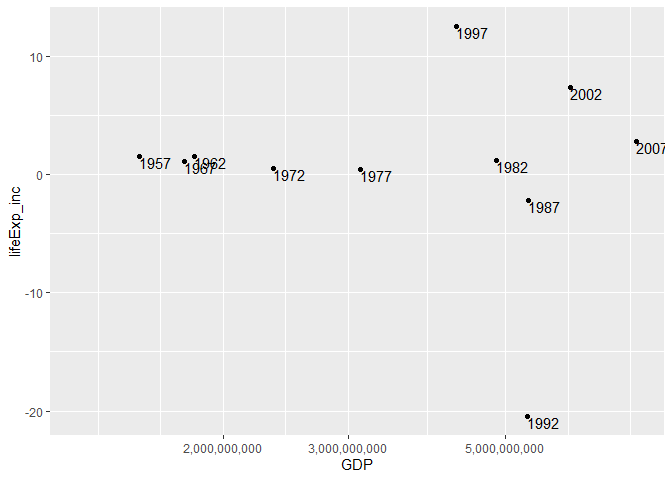
\includegraphics{hw03_files/figure-latex/unnamed-chunk-4-1.pdf}


\end{document}
